\documentclass[11pt,a4paper]{article}
\usepackage[margin=24mm]{geometry}
\usepackage{amsmath,amssymb,graphicx,booktabs,array}
\usepackage[colorlinks=true,allcolors=blue]{hyperref}
\usepackage{microtype}
\newcommand{\pt}{p_{\mathrm T}}
\newcommand{\AUC}{\operatorname{AUC}}
\newcommand{\E}{\mathbb E}
\setlength{\emergencystretch}{2em}
\renewcommand{\topfraction}{.9}
\renewcommand{\bottomfraction}{.8}
\renewcommand{\textfraction}{.08}
\renewcommand{\floatpagefraction}{.75}
\raggedbottom
\title{Contrastive Pretraining on Real LHC Jets:\\Transfer, Scorer Dependence and Mass Distortion}
\author{Animesh Parashar$^1$ \and Aditya Parashar$^2$}
\date{3 October 2026}
\begin{document}
\maketitle
\begin{center}\small
$^1$Department of Physics, IIT (ISM) Dhanbad, Dhanbad 826004, Jharkhand, India\\
$^2$Department of Computer Science and Engineering, BIT Mesra, Ranchi 835215, India
\end{center}
\begin{abstract}
We compare contrastive pretraining on real AspenOpenJets and simulated LHC Olympics
jets for background-based anomaly ranking, using matched random backbones and jet
observables as controls. Equal training budgets comprise 100,000 jets per domain,
one real-data shard and three seeds. Only 24 real-data training jets lie in the
simulated reference sample's central 90\% transverse-momentum range, preventing a
causal attribution to the pretraining domain. On partitions withheld from
development, transverse-momentum balancing gives mean nearest-neighbor AUCs of
0.541, 0.564 and 0.517 for real-data, simulation and random representations on
two-prong signals; three-prong values are 0.419, 0.553 and 0.426. All real-data seeds
rank three-prong signal below background. Random backbones lead the original
two-prong comparison with mean AUC 0.636. Signal--background momentum and
multiplicity differences are consistent with score correlations and ranking
changes, without establishing their cause. Regularized Mahalanobis and whitened
nearest-neighbor scores do not make real-data representations competitive with
girth; whitening benefits random features more. At background-calibrated operating
points, girth retains more signal but strongly distorts background jet mass,
whereas real-data-trained scores retain little signal. This bounded comparison
characterizes representation, scorer and population dependence. Prior access to
these public benchmarks limits independence; scorer and physics extensions are
post-evaluation diagnostics.
\end{abstract}

\section{Introduction and scope}
Learning from real collision data is attractive when simulated backgrounds do
not fully reproduce detector response and jet structure. However, a useful
representation need not induce a useful anomaly ranking under a particular
metric. A comparison of pretraining domains must therefore distinguish the
representation, its readout, the evaluation population and optimization variability.

JetCLR established symmetry-informed contrastive jet representations and linear
classifier tests~\cite{jetclr}. Contrastive dijet representations and weakly
supervised anomaly searches were investigated in Ref.~\cite{dillon2022}; AnomalyCLR
uses anomaly-oriented augmentations and latent reconstruction scoring~\cite{anomalyclr}.
AspenOpenJets demonstrates beneficial real-data pretraining for generative transfer
with OmniJet-$\alpha$~\cite{aspen,omnijet}; that task differs from background-referenced
anomaly ranking. OmniLearned demonstrates anomaly detection with CMS experimental
data using large-scale multitask pretraining~\cite{omnilearned}. Metzger et al.
show that representations optimal for background classification need not maximize
new-physics sensitivity~\cite{metzger}; our readout-dependent findings are a bounded
example of this distinction, not its first observation. We claim neither
first discriminative use of AspenOpenJets nor a new contrastive objective.
Related self-supervised approaches use re-simulation to define alternative views
(RS3L)~\cite{rs3l} or recover masked particles~\cite{mpm}. These extend the range
of pretraining strategies; the present rotation-only comparison does not test them.

We ask a narrower question: under a specified equal-sample, equal-update recipe,
does real-data pretraining improve simulated-signal ranking relative to simulation
pretraining and matched random initialization? We then test how the answer depends
on two established covariance-based scorers and on physically relevant operating
points. Mass distortion matters because selection can reshape background spectra,
a concern already studied in jet tagging and anomaly detection~\cite{ddt,massive}.
Distance-correlation regularization provides an established route to reducing
such dependence~\cite{disco}; no mass-decorrelated control is implemented here.
Our contribution is the combined empirical characterization of domain, seed,
scorer and retention--distortion behavior in this particular transfer setting.
The latter two analyses were specified after inspecting the fixed-score results.
They broaden the characterization, not the independence of its evidence.
The principal findings are:
\begin{enumerate}
\item The compared training distributions have little overlap in their dominant
momentum ranges; the observed transfer result does not identify a domain cause.
\item No stable Aspen advantage emerges across three seeds; its three-prong
raw-score ranking is inverted for every seed.
\item Whitening benefits matched random features more than Aspen features,
while supervised probes reveal information not recovered by these anomaly scores.
\item Girth retains substantially more signal but strongly sculpts background
jet mass; weak sculpting without signal retention is insufficient.
\end{enumerate}

\section{Datasets, representation and separation}
\subsection{Inputs and physical definitions}
AspenOpenJets is derived from CMS 2016 Open Data~\cite{aspen}. We use the available
\texttt{RunG\_batch0.h5} shard and its stored jet constituents, with at most 150
constituents supplied per jet. The selected training sample contains 100,000 jets;
it is unlabeled and not certified background-only. We do not use impact parameters,
charge or constituent pileup weights in this comparison.
The producer selects anti-$k_t$ $R=0.8$ jets with corrected $\pt>300$\,GeV and
$|\eta|<2.5$ from the JetHT stream, an inclusive combination of hadronic triggers,
with standard event/jet quality requirements. Its jet reconstruction uses PUPPI
and jet-energy corrections~\cite{aspen}. Our sums of stored, unweighted constituents
are not those corrected producer jet quantities.

The LHC Olympics R\&D sample~\cite{lhco,lhcocommunity} contains one million QCD events and
100,000 two-prong signal events. Its $W'\to XY$ benchmark has masses
$(m_{W'},m_X,m_Y)=(3500,500,100)\,\mathrm{GeV}$ and $X,Y\to qq$ decays.
A separate 100,000-event sample uses $X,Y\to qqq$ with otherwise corresponding
generator settings. The samples use Pythia8 and Delphes 3.4.1 without pileup or
multiple-parton interactions and were selected with an $R=1$ fat-jet trigger at
$\pt>1.2\,\mathrm{TeV}$~\cite{lhco}. Our subsequent $R=0.8$ leading-jet analysis
is a specified adaptation, not a reproduction of the producer's $R=1$ features.

For simulated events, massless particle inputs $(\pt,\eta,\phi)$ are converted to
four-vectors and clustered with FastJet anti-$k_t$, $R=0.8$, using E-scheme
recombination~\cite{antikt,fastjet}. We choose the jet with largest vector $\pt$.
Aspen inputs retain the producer's stored constituent membership. For either
domain, let $P^\mu=\sum_{i\in J}p_i^\mu$ over all available jet constituents and
$S_T=\sum_{i\in J}p_{\mathrm T,i}$. The axis is defined by
\begin{equation}
 p_{\mathrm T,J}=\sqrt{P_x^2+P_y^2},\qquad
 \eta_J=\operatorname{arsinh}(P_z/p_{\mathrm T,J}),\qquad
 \phi_J=\operatorname{atan2}(P_y,P_x).
\end{equation}
Before truncation, each constituent is represented as
\begin{equation}\label{eq:features}
 x_i=\left(\eta_i-\eta_J,\;\operatorname{wrap}_{[-\pi,\pi)}(\phi_i-\phi_J),\;
 \log\frac{p_{\mathrm T,i}}{S_T},\;\log\frac{p_{\mathrm T,i}}{\mathrm{GeV}}\right).
\end{equation}
We retain the 50 highest-$\pt$ constituents and explicitly mask padding.
The full axis and denominator are not recomputed after truncation. Full-jet mass
is $m_J=\sqrt{\max(0,P_\mu P^\mu)}$; full multiplicity counts available nonzero-$\pt$
constituents before truncation. Shared feature definitions do not equalize
selection, physics composition, pileup or detector response across domains.
Only 3/100,000 selected Aspen training jets have 150 nonzero stored constituents.
This measures saturation of the stored list, not a truth-level truncation-loss
rate. Signal labels identify events rather than a truth-matched leading $X$ or
$Y$ jet; Appendix~\ref{app:diagnostics} shows the leading-jet mass distributions.

\subsection{Partitions and data exposure}
Event-identity hashing assigns background or unlabeled events to training,
validation, reference and test partitions with nominal fractions 60/15/10/15.
Signals have only validation/test partitions, nominally 50/50. Events examined
during initial data checks are assigned to validation. Aspen jets sharing an
event identity share a partition. Training loaders reject signal, reference and
test inputs. Both domains use fixed samples of 100,000 training and 8,192 validation
jets; samples are identical across training seeds within each domain.
Those checks covered 5120 Aspen jet rows from 3164 distinct events and 5120 LHCO
events (4608 background and 512 signal). Their identities are reserved for
validation, including other Aspen jets from an examined event.

Development evaluation uses 10,000 background validation references, 10,000
distinct background validation queries and 2,000 signal queries. The frozen
final-partition evaluation uses 10,000 background reference events, 10,000
background test events and 2,000 signal test events per topology. Both final
topologies share the same background events. Three-prong source IDs occupy a
distinct namespace; 49,945/50,055 events enter validation/test, with no rejected
rows and no overlap. Each simulated query is one leading jet per event.

Here ``final'' means withheld from the development of this pipeline. The public
benchmarks were accessible before the final evaluation, so the final partitions
do not provide fully independent confirmation. Development was adaptive, including inspection of
signal-validation scores. The final protocol was fixed before the reported
final-partition scoring, but subsequent scorer and physics extensions were
motivated by those results. No independent discovery dataset is claimed.

\subsection{Kinematic support of the training samples}\label{sec:support}
After the primary evaluation, we reconstructed the exact training-row selections
from the completed run manifests and compared them with the fixed background references
(Fig.~\ref{fig:support}). The available-constituent vector-$\pt$ medians are
336.8\,GeV for Aspen training, 1310.9\,GeV for simulation training and 1307.9\,GeV
for simulation references. Of 100,000 training jets, only 24 Aspen jets and
89,592 simulation jets lie in the reference central 90\% range,
$[1198.6,1740.9]$\,GeV. All reference jets lie outside Aspen training's central
98\% range $[257.5,706.9]$\,GeV. Central ranges describe concentration, not strict
support; rare Aspen jets do extend into the evaluation regime.

The features explicitly retain the scalar momentum scale because
$x_{i,4}-x_{i,3}=\log(S_T/\mathrm{GeV})$. Evaluation-time balancing of signal and
background does not match the pretraining domains. These measurements establish
a major distribution mismatch, but do not determine how much of the ranking
deficit it causes. Removing the absolute-momentum input would test explicit scale
dependence without equalizing detector response, composition or all kinematic
correlations.
\begin{figure}[tbp]\centering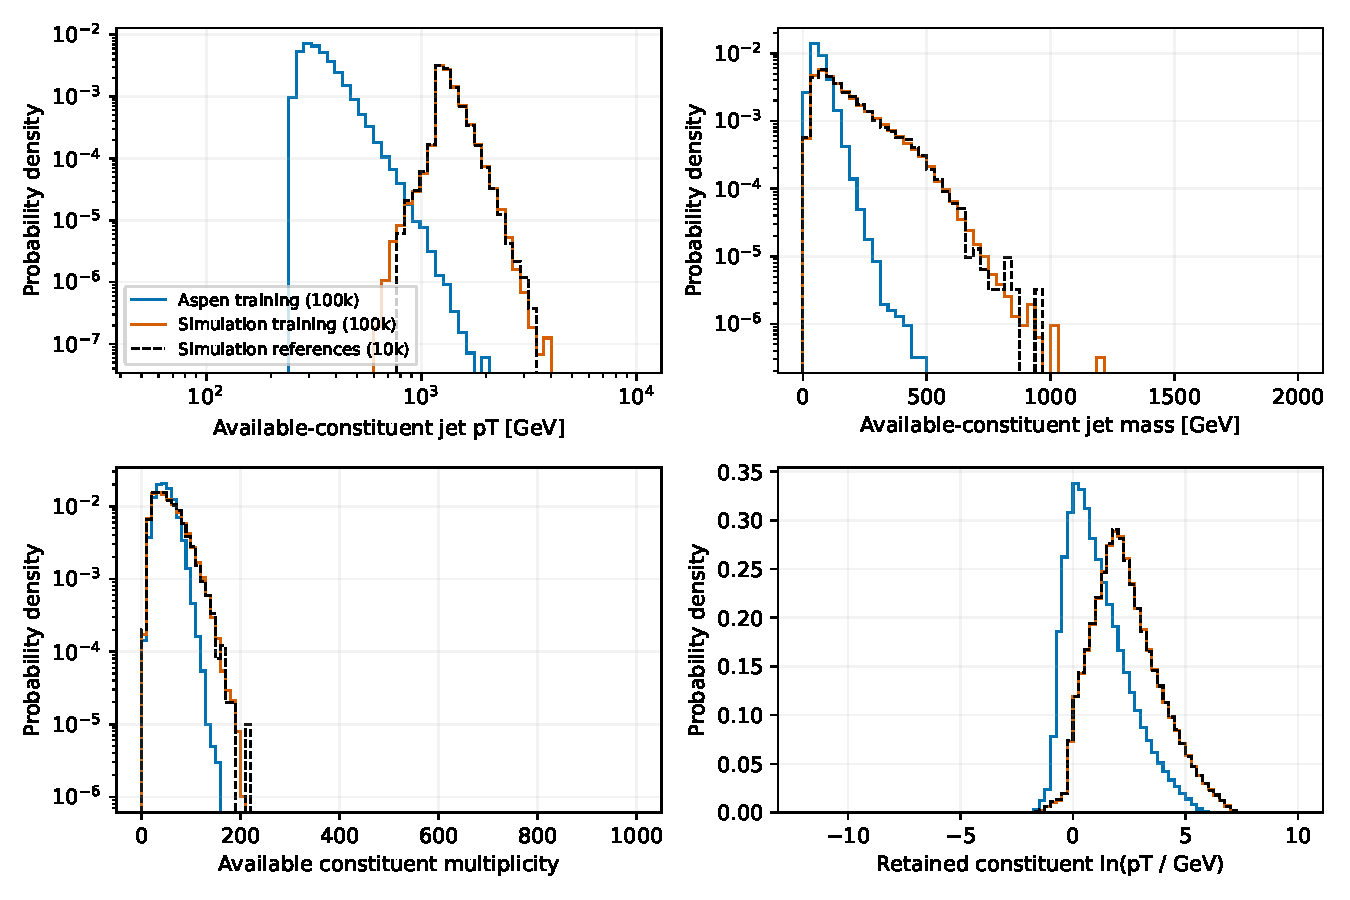
\includegraphics[width=.82\linewidth]{figures/training_support.pdf}
\caption{Exact selected training samples and fixed simulation references.
Jet quantities use all available constituents; the constituent-momentum panel
uses the retained 50 or fewer, with equal total weight per jet. Histograms retain
their full-population normalization; underflow/overflow probabilities and
particle-weighted alternatives are supplied in the numerical supplement.}
\label{fig:support}\end{figure}

\section{Models, learning and scoring}
\subsection{Encoder and optimization}
The backbone consists of a four-feature linear input map, four independently
initialized pre-normalized Transformer encoder layers~\cite{attention} with width
128, eight heads, feed-forward width 512, ReLU activations and dropout 0.1, followed
by layer normalization and masked mean pooling. Input features are divided by
$(1,1,5,5)$. With no positional encoding and masked mean pooling, the deterministic
evaluation backbone is permutation-invariant up to numerical roundoff.
A $128\to128\to256$ projection head
with an intermediate GELU and final unit normalization is used only for training.

Two independently sampled local $(\Delta\eta,\Delta\phi)$ rotations, with angles
uniform in $[-\pi,\pi]$, define positive views. The momentum features are unchanged.
The implemented $\phi$-chart rejection rule never triggers in the selected training
samples: maximum local radii are 1.192 (Aspen) and 1.153 (simulation), both below
$\pi$. This planar transformation approximates a narrow-jet augmentation; it is
not an exact Lorentz/global-azimuth symmetry and need not preserve exact jet mass.
No exact infrared/collinear safety is asserted for the finite, truncated network.
Rotation-only views define a restricted recipe inspired by JetCLR, not a
reproduction of its full augmentation study.

For $B=128$ jets and $2B$ normalized projections $u_i$, paired-view index $p(i)$,
the symmetric normalized temperature-scaled cross-entropy~\cite{simclr} is
\begin{equation}
 \mathcal L=-\frac{1}{2B}\sum_{i=1}^{2B}
 \log\frac{\exp(u_i^Tu_{p(i)}/\tau)}{\sum_{j\ne i}\exp(u_i^Tu_j/\tau)},\qquad\tau=0.1.
\end{equation}
The positive is included in the denominator; only self-similarity is excluded.
AdamW~\cite{adamw} uses learning rate $3\times10^{-4}$, weight decay $10^{-4}$ and
gradient-norm clipping at 1. We train for 100 epochs without a learning-rate
schedule and with dropped incomplete batches (781 updates/epoch). Validation
views are fixed for loss monitoring; no signal-AUC endpoint selection is used.
Seeds 17, 29 and 43 have matched initial backbones across domains. Random controls
are their saved initial backbones, not separately tuned models. Seed 17 was
continued from saved optimizer/RNG state to the fixed endpoint; the completed
seed-43 runs use the original trainer from initialization after a walltime-limited
attempt was discarded. Partial results are not selected or combined.
The final fixed-view validation losses span 0.0208--0.0214 across the six runs;
their histories appear in Appendix~\ref{app:diagnostics}. Similar endpoint losses
do not establish similar representation or anomaly-ranking quality.

\subsection{Frozen score and controls}
Scoring uses raw 128-dimensional backbone outputs $h(x)$, not the normalized
projection head. For background reference embeddings $\mathcal R$, the original
score is
\begin{equation}s_{10}(x)=\operatorname{kth}_{10}\{\|h(x)-r\|_2:r\in\mathcal R\},\end{equation}
with larger scores designated anomalous. It is the tenth distance, not the mean
of ten distances. AUCs below 0.5 are retained without reversing the score.
Reference size 10,000 and $k=10$ are fixed choices; their sensitivity is not tested.

Controls include high mass, high $\pt$, both signs of multiplicity, high girth,
and tenth-neighbor distance in $(m_J,p_{\mathrm T,J},n_J,g_J)$ after background-reference
mean/standard-deviation scaling. Girth is
\begin{equation}
 g_J=\frac{\sum_{i\in J_{50}}p_{\mathrm T,i}\sqrt{(\Delta\eta_i)^2+(\Delta\phi_i)^2}}
 {\sum_{i\in J_{50}}p_{\mathrm T,i}},
\end{equation}
using retained constituents relative to the full axis. It is not a full-jet girth.
The observable-density control has access to full mass and multiplicity, so it is
not an information-matched learned-representation comparison. Girth is computable
from the encoder inputs. These controls test practical value rather than claim
a matched optimization of all possible physics taggers.

\subsection{Subsequent covariance-scorer extension}
For each backbone, background references alone fit
\begin{equation}
 \mu=\frac{1}{N}\sum r_i,\quad C=\frac{1}{N}\sum(r_i-\mu)(r_i-\mu)^T,\quad
 C_\lambda=0.9C+0.1\frac{\operatorname{tr}C}{128}I.
\end{equation}
With $C_\lambda=LL^T$, column vectors transform as $z=L^{-1}(h-\mu)$.
We evaluate $s_M=\|z\|^2$ and tenth-neighbor distance in transformed coordinates.
Regularization, $k$, models and score signs are fixed before this extension;
there is no hyperparameter search. The regularized covariance, not necessarily
the empirical covariance, whitens to identity. Mahalanobis distance is not a
calibrated tail probability. All 27 backbone/scorer combinations per topology
are reported. The extension is descriptive post-evaluation robustness analysis.

\section{Evaluation and uncertainty}
\subsection{AUC and kinematic support}
We report original-population AUC alongside a common-$\pt$ diagnostic. Twenty
background-reference quantile bins define edges. Bins must contain at least 30
queries of each class and lie within reference support. For class $c$ in supported
bin $b$, the event weight is
\begin{equation}
 w_i=\frac{\min(n_{0b},n_{1b})}{n_{cb}},\quad i\in(c,b);
 \qquad w_i=0\text{ otherwise}.
\end{equation}
Weighted AUC is the weighted signal--background pair average of
$\mathbf 1[s_S>s_B]+\tfrac12\mathbf 1[s_S=s_B]$, normalized by the product of
class weight sums. This equalizes coarse $\pt$-bin class masses, not within-bin
kinematics or other confounders. It uses evaluation labels and is not a deployment
selection. The final comparison excludes 5,468/10,000 background queries and
186/2,000 two-prong or 180/2,000 three-prong signals. Effective sizes
$(\sum w)^2/\sum w^2$ are approximately 2,329/1,789 and 2,371/1,775 for the two
background/signal pairs. Thus balanced and original AUCs describe materially
different populations and must be presented together.
For both topologies, supported bins are reference quantile bins 12--20
(one-based), spanning approximately 1327.1--3223.1\,GeV; exact edges and counts
are supplied with the diagnostic results.

Three-seed arithmetic means and sample SDs refer to individual-model metrics,
not averaged-score ensembles. Domain differences are paired by seed. Shared,
class-stratified event bootstraps (1,000 replicates) recompute the balancing
weights with fixed edges. Their percentile intervals condition on fitted models
and reference events; they exclude training and reference-fitting uncertainty.
They cannot substitute for seed variability. Later extensions use pointwise
intervals without multiplicity-adjusted confirmatory claims. Failure to establish
an advantage is not evidence of equivalence.

\subsection{Background-calibrated physics diagnostic}
The 10,000 shared background queries are split once into disjoint 5,000-event
calibration and assessment sets. For target background acceptance $a\in\{0.10,0.05\}$,
the threshold is the $\lceil5000a\rceil$-th largest calibration score; selections
include all ties. All 2,000 signals of each topology assess efficiency. No signal
enters threshold fitting. This uses original, unweighted populations, and actual
assessment acceptance is reported rather than assumed equal to the target.

Let $F$ and $F_{\rm sel}$ be inclusive and selected assessment-background mass
CDFs. We measure $D_{\rm KS}=\sup_m|F(m)-F_{\rm sel}(m)|$ without an independent-sample
KS $p$-value: selected events are a subset of the inclusive sample. We also use
\begin{equation}
 \operatorname{JSD}(p,q)=\tfrac12\sum_b p_b\log\frac{p_b}{(p_b+q_b)/2}
 +\tfrac12\sum_b q_b\log\frac{q_b}{(p_b+q_b)/2},
\end{equation}
for normalized ten-bin mass histograms. Bins are calibration-background quantiles,
with outer edges extended to infinity, no pseudocounts, and $0\log0=0$. JSD is
in natural-log units. Empty selected samples would yield undefined shape metrics,
not zero distortion. Marginal acceptance profiles use analogous mass and $\pt$
bins. They do not measure mass dependence conditional on $\pt$.

Finite samples create apparent distortion even for mass-neutral selection.
Five hundred uniform subsets of the assessment background, matched to each
observed selected count, provide descriptive KS/JSD reference bands. These are
not discovery $p$-values. Conditional binomial uncertainty uses Wilson intervals~\cite{wilson};
1,000 paired bootstraps additionally resample calibration background, assessment
background and each signal class independently and refit thresholds in every
replicate. The selected/inclusive nesting and ties are preserved. Models,
reference fits, bins and the event split remain fixed. Both topologies share
background events and are not independent experimental confirmations.

\section{Results}
\subsection{Transfer and seed variation}
Table~\ref{tab:final} and Fig.~\ref{fig:auc} show the frozen final-partition comparison.
Two-prong common-$\pt$ Aspen-minus-simulation differences are $-0.0789,+0.0965,-0.0872$
for seeds 17, 29 and 43. Their mean is $-0.0232$ with sample SD $0.1038$; the
fixed-model event-bootstrap interval $[-0.0448,-0.0026]$ conditions on these three
trained models and the reference events. It excludes training variability and
therefore is not evidence for a reproducible domain difference. No stable domain
advantage is established.
In the original population, high $\pt$ alone has AUC 0.833 (two-prong) and
0.835 (three-prong), exceeding every learned score in this comparison. After
common-$\pt$ balancing its AUC is approximately 0.494--0.495, as expected when
coarse momentum differences are removed.
For three-prong signals all three Aspen raw-score balanced AUCs are below 0.5.
This is inverted ranking under the prescribed score direction, not proof that
all signal information is absent. Girth exceeds every trained seed in the balanced
population on both topologies.
\begin{table}[htbp]\centering\scriptsize
\resizebox{\linewidth}{!}{\begin{tabular}{lrrrr}
\toprule
Score & 2p original & 2p balanced & 3p original & 3p balanced \\
\midrule
Aspen & $0.5114\pm0.0626$ & $0.5407\pm0.0391$ & $0.3968\pm0.0534$ & $0.4188\pm0.0317$ \\
Simulation & $0.5504\pm0.2170$ & $0.5639\pm0.0672$ & $0.5446\pm0.2219$ & $0.5528\pm0.0848$ \\
Random & $0.6361\pm0.0164$ & $0.5172\pm0.0174$ & $0.5580\pm0.0168$ & $0.4255\pm0.0160$ \\
High mass & 0.6390 & 0.6065 & 0.6637 & 0.6322 \\
High $p_T$ & 0.8334 & 0.4940 & 0.8353 & 0.4948 \\
High multiplicity & 0.4265 & 0.4301 & 0.5744 & 0.5770 \\
Low multiplicity & 0.5735 & 0.5699 & 0.4256 & 0.4230 \\
Girth & 0.6858 & 0.7131 & 0.6838 & 0.7118 \\
Observable density & 0.8095 & 0.6452 & 0.7691 & 0.6060 \\
\bottomrule
\end{tabular}
}
\caption{Primary frozen-score final-partition AUCs; 2p and 3p denote two-prong and
three-prong signals. Model entries are mean $\pm$ sample SD over
three training/initialization seeds, not confidence intervals. Physics controls
have no encoder seeds. ``Balanced'' denotes the restricted common-$\pt$ population.}
\label{tab:final}\end{table}
\begin{figure}[htbp]\centering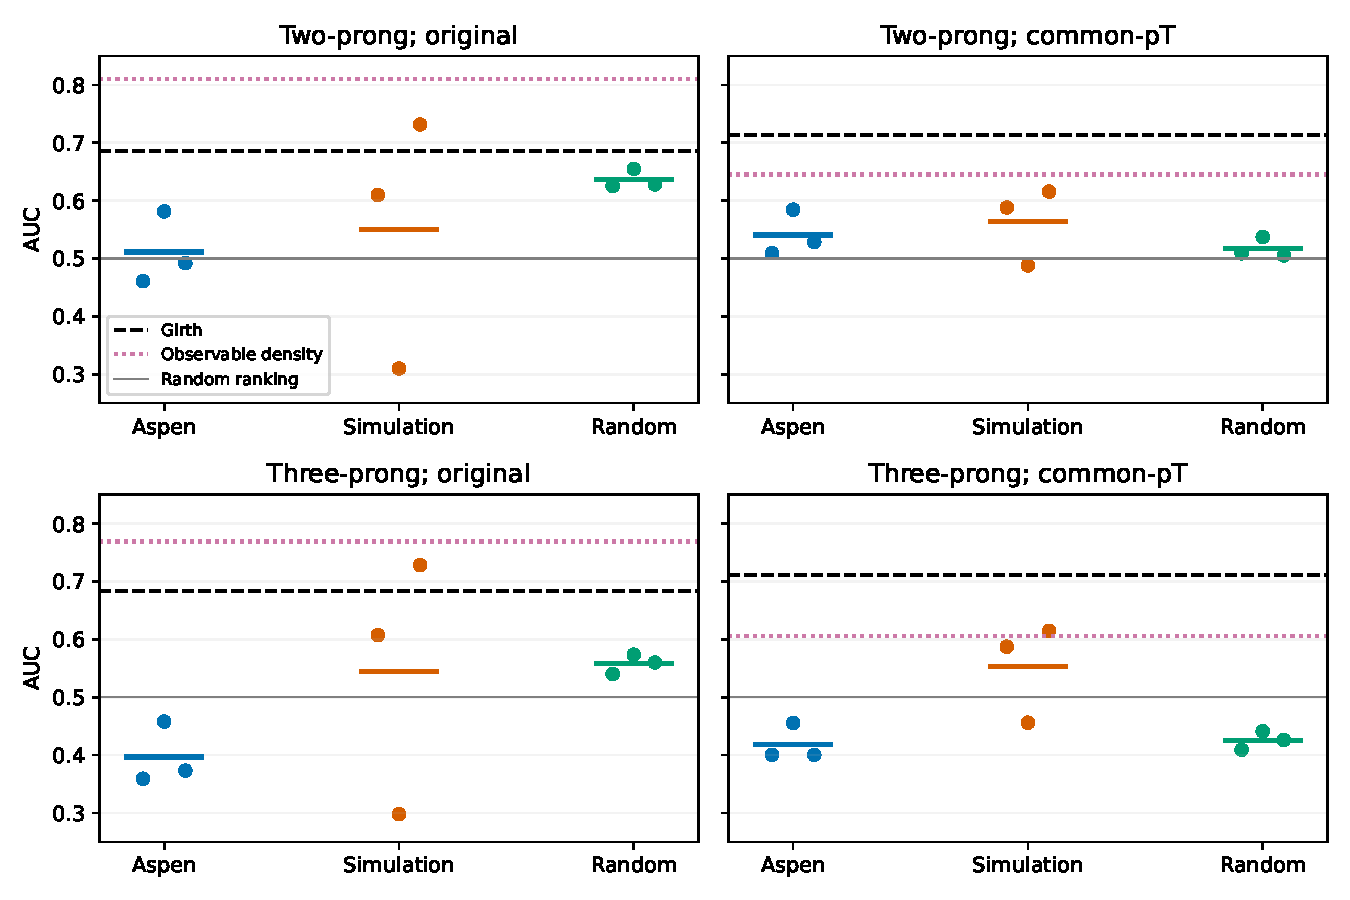
\includegraphics[width=.95\linewidth]{figures/auc_seeds.pdf}
\caption{Each point is one seed; short bars show seed means. Dashed/dotted lines
are physics controls. Both the population definition and initialization materially
change the apparent ranking. No seed is discarded.}\label{fig:auc}\end{figure}

\subsection{Dependence on the scorer}
The subsequent scorer comparison is given in Table~\ref{tab:scorers} and
Fig.~\ref{fig:scorers}. Whitening changes Aspen common-$\pt$ mean AUC by $+0.0019$
(two-prong) and $-0.0087$ (three-prong), compared with $+0.0470$ and $+0.0478$ for
random backbones. On two-prong queries, the Aspen-minus-random difference changes
from $+0.0235$ under raw kNN to $-0.0217$ under whitened kNN and $-0.0281$ under
Mahalanobis scoring. An improvement after metric adjustment cannot therefore be
attributed to learning without the corresponding random-feature control.
Simulation improves modestly under whitening, with substantial seed variability.
Every trained seed/scorer remains below girth in both balanced populations.
These findings extend the weak result beyond raw Euclidean kNN but do not test
all anomaly scores or configurations.
\begin{table}[htbp]\centering\scriptsize
\resizebox{\linewidth}{!}{\begin{tabular}{llrrrr}
\toprule
Backbone & Scorer & 2p original & 2p balanced & 3p original & 3p balanced \\
\midrule
Aspen & Raw kNN & $0.5114\pm0.0626$ & $0.5407\pm0.0391$ & $0.3968\pm0.0534$ & $0.4188\pm0.0317$ \\
Aspen & Mahalanobis & $0.4664\pm0.0353$ & $0.5182\pm0.0097$ & $0.3678\pm0.0330$ & $0.4162\pm0.0137$ \\
Aspen & Whitened kNN & $0.5078\pm0.0532$ & $0.5426\pm0.0225$ & $0.3843\pm0.0527$ & $0.4101\pm0.0233$ \\
Simulation & Raw kNN & $0.5504\pm0.2170$ & $0.5639\pm0.0672$ & $0.5446\pm0.2219$ & $0.5528\pm0.0848$ \\
Simulation & Mahalanobis & $0.5555\pm0.1886$ & $0.5591\pm0.0706$ & $0.5518\pm0.2017$ & $0.5596\pm0.0908$ \\
Simulation & Whitened kNN & $0.5653\pm0.1962$ & $0.5849\pm0.0711$ & $0.5538\pm0.2054$ & $0.5698\pm0.0904$ \\
Random & Raw kNN & $0.6361\pm0.0164$ & $0.5172\pm0.0174$ & $0.5580\pm0.0168$ & $0.4255\pm0.0160$ \\
Random & Mahalanobis & $0.6366\pm0.0086$ & $0.5463\pm0.0106$ & $0.5598\pm0.0070$ & $0.4623\pm0.0123$ \\
Random & Whitened kNN & $0.6296\pm0.0141$ & $0.5642\pm0.0132$ & $0.5420\pm0.0094$ & $0.4733\pm0.0100$ \\
\bottomrule
\end{tabular}
}
\caption{All fixed scorers on original and common-$\pt$ populations, mean $\pm$
seed SD. This comparison was added after the primary final-score evaluation.}
\label{tab:scorers}\end{table}
\begin{figure}[htbp]\centering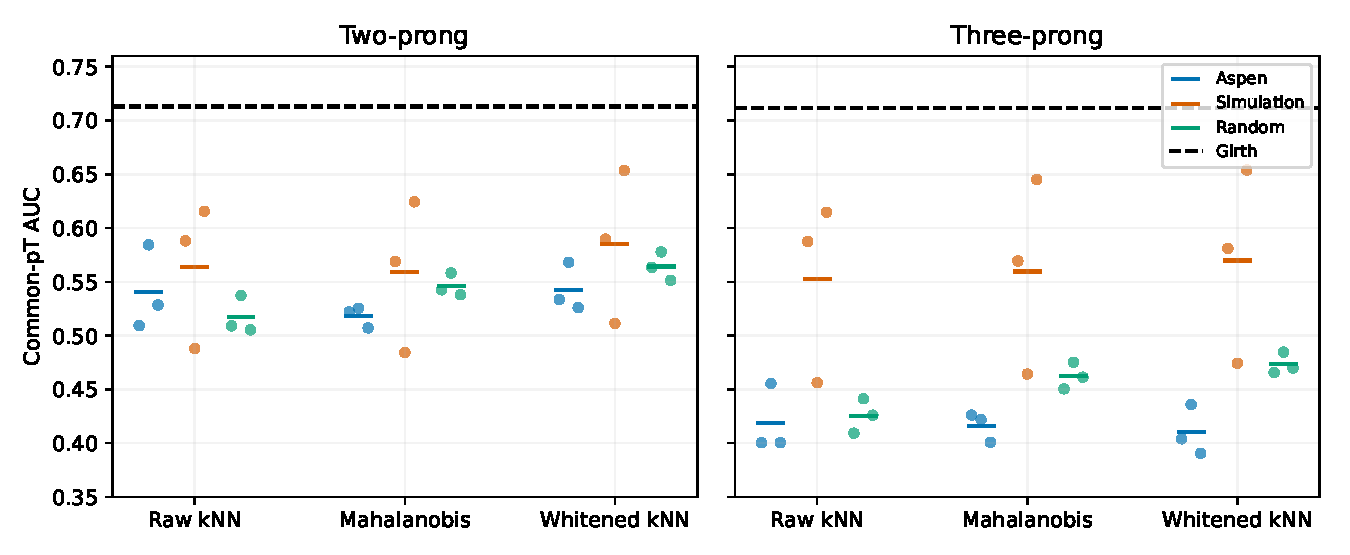
\includegraphics[width=.95\linewidth]{figures/scorer_sensitivity.pdf}
\caption{Common-$\pt$ scorer sensitivity. Short horizontal markers show seed
means; offset points show every seed. Scorers are discrete fixed choices.}
\label{fig:scorers}\end{figure}

\subsection{Signal retention versus mass distortion}
At nominal 5\% background acceptance, raw Aspen has actual mean acceptance 5.53\%,
retains 3.17\%/0.92\% of two-/three-prong signals, and has mean mass KS distance
0.135. Girth has actual acceptance 4.82\%, retains 24.10\%/22.05\%, and has KS
0.893. Observable density has acceptance 4.74\%, retains 31.85\%/30.30\%, and has
KS 0.586. Raw simulation lies between these examples with 4.95\% acceptance,
9.75\%/9.68\% retention and KS 0.318, but its signal-efficiency seed SDs are
9.15/8.59 percentage points. Actual acceptance differences and training variation
must accompany the comparison.

Girth's stronger retention comes with pronounced mass sculpting. Its 241 selected
assessment-background events at nominal 5\% give KS 0.893, versus a count-matched
random-selection reference range approximately $[0.029,0.093]$. Conversely,
Aspen's weaker distortion comes with mean signal acceptance below mean background
acceptance for every tested scorer and both operating points. A signal-independent
random selection would retain equal fractions in expectation. Weak sculpting
alone does not establish a useful anomaly tagger. Neither spectrum distortion
nor these efficiencies establish a fake resonance, sideband-fit bias or discovery
significance. The measured mass is jet mass, not dijet mass.
KS is a marginal diagnostic and includes distortion induced by $\pt$ selection.
No mass-decorrelated tagger or optimal retention--distortion frontier is claimed.
\begin{table}[htbp]\centering\small
\resizebox{\linewidth}{!}{\begin{tabular}{lrr}
\toprule
Raw-score backbone & Selected background counts (seeds 17, 29, 43) & Total \\
\midrule
Aspen & 269, 284, 277 & 5000 \\
Simulation & 238, 246, 258 & 5000 \\
Random & 267, 259, 264 & 5000 \\
\bottomrule
\end{tabular}
}
\caption{Raw-score selected assessment-background counts at nominal 5\%.
Girth selects 241 and observable density 237 of the same 5000 events. All scorer
counts and achieved rates are supplied in the numerical supplement.}
\end{table}
\begin{figure}[htbp]\centering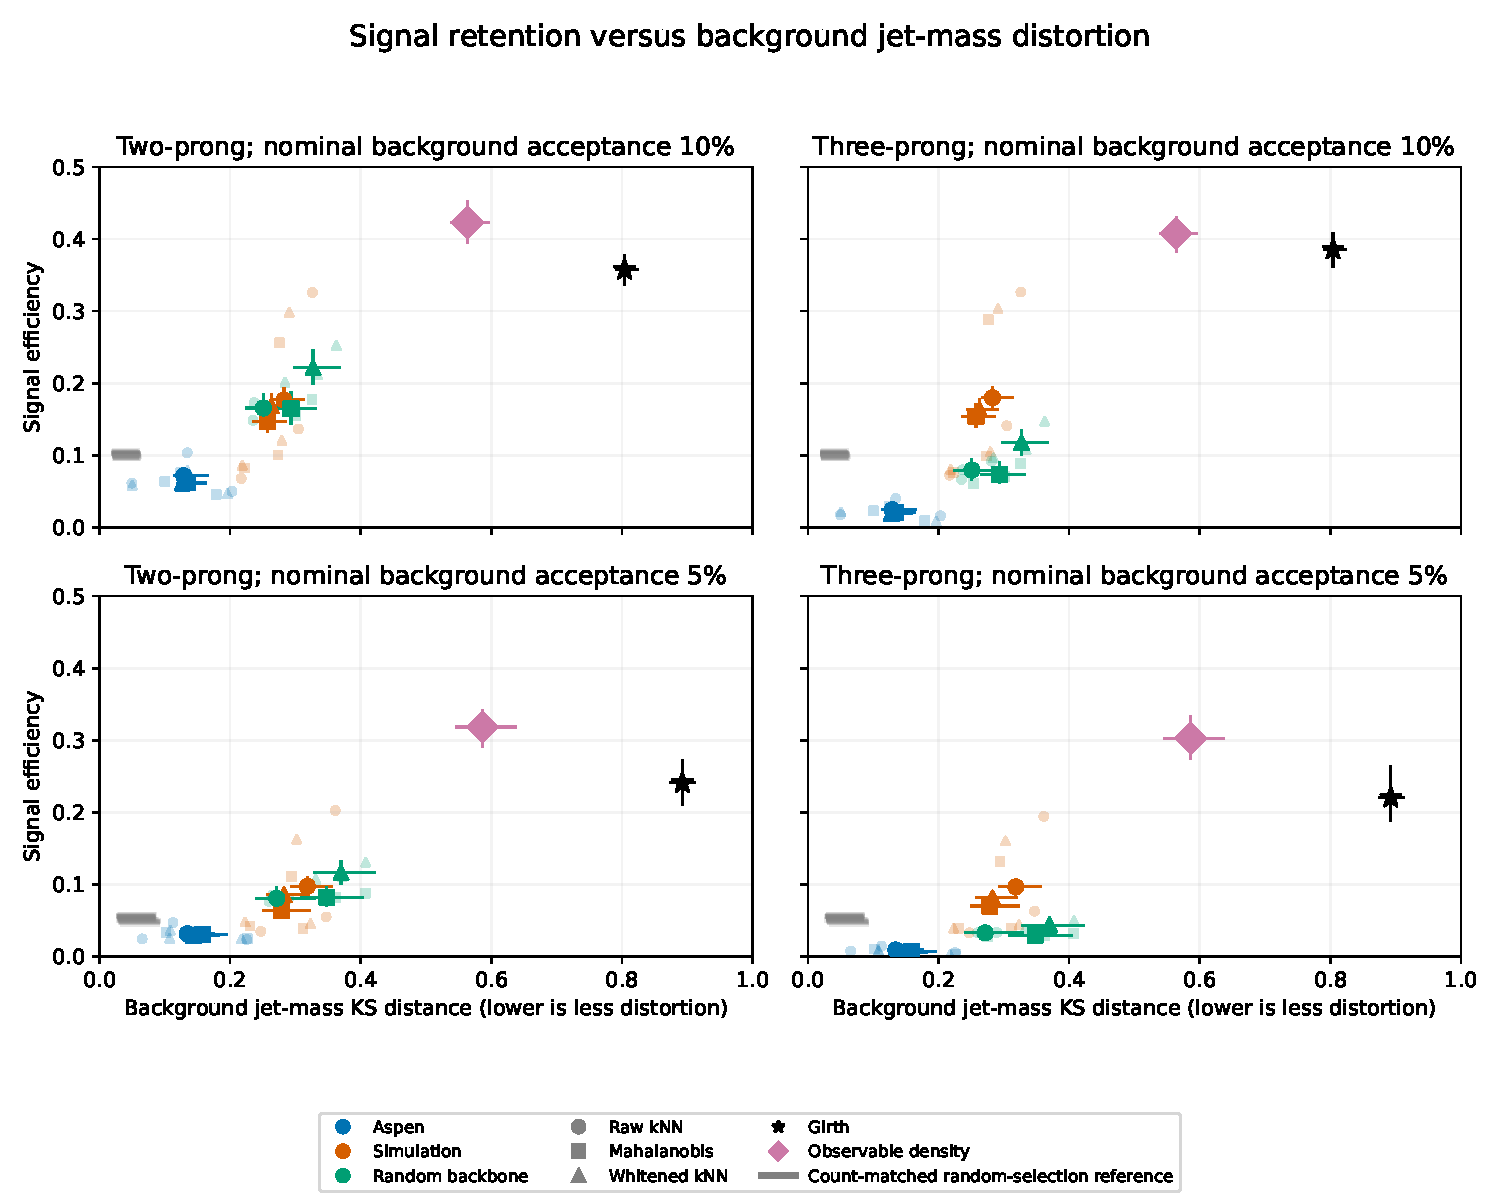
\includegraphics[width=.95\linewidth]{figures/physics_tradeoff.pdf}
\caption{Signal retention versus background jet-mass distortion. Large model
markers show three-seed means and faint points show individual seeds; shape
identifies the scorer. Horizontal/vertical segments are marginal 95\% event-bootstrap
intervals with threshold refitting, conditional on trained models and references;
they are not joint regions or training uncertainty. Gray segments show each arm's
count-matched random-selection KS band at its achieved background acceptance,
the expected signal efficiency of an independent random selection. These are
reference expectations, not measured random-cut signal efficiencies. All values
use unweighted populations; nominal rates are in titles and achieved rates in
Appendix~\ref{app:tables}.}
\label{fig:tradeoff}\end{figure}
\begin{figure}[htbp]\centering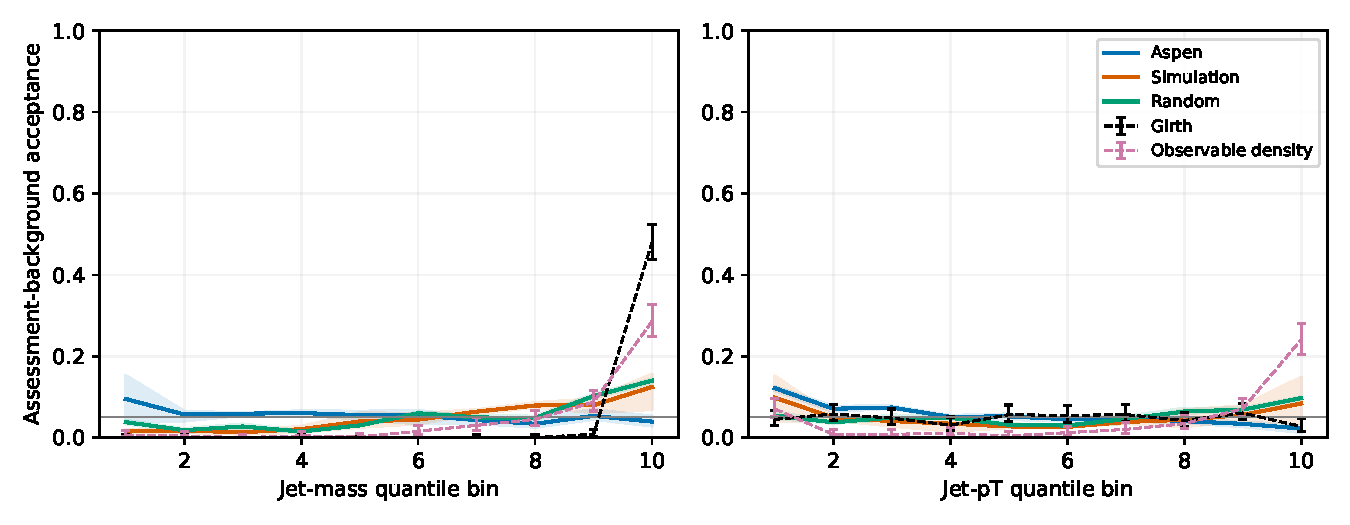
\includegraphics[width=.95\linewidth]{figures/acceptance_profiles.pdf}
\caption{Background acceptance versus calibration-defined mass and $\pt$ quantile
bins at nominal 5\%. Raw-score curves show seed means and shaded seed minima/maxima,
not confidence bands. Controls show fixed-threshold 95\% Wilson intervals.
Outer bins include overflow. These marginal profiles do not isolate mass effects
at fixed $\pt$. Conditional binomial intervals for all profiles are supplied
in the numerical supplement.}\label{fig:profiles}\end{figure}

\subsection{Representation geometry and score correlations}\label{sec:representation}
We use the cached embeddings of all nine frozen backbones to characterize their
geometry and their dependence on elementary jet observables.
On 10,000 background queries, raw Aspen scores anticorrelate with available
multiplicity (Spearman $\rho=-0.53$ to $-0.58$). Simulation's score--$\pt$
correlation changes from $-0.436$ for seed 29 to $+0.289$ for seed 43.
These associations are consistent with sensitivity to jet-level properties,
and the evaluated populations clarify their possible relevance
(Fig.~\ref{fig:signal_kinematics}). Original signal momentum medians are
1645.7 and 1644.7\,GeV for two- and three-prong jets, compared with
1309.7\,GeV for background. Increasing momentum alone gives AUCs 0.833 and 0.835,
falling to 0.494 and 0.495 after the existing coarse-bin balancing. The harder
signals are consistent with the ordering of simulation seeds 29 and 43 by their
score--momentum correlation and original two-prong AUC (0.31 versus 0.73).
This is an association, not a decomposition of the learned score.

Multiplicity differs in opposite directions: original medians are 41 for
two-prong signal, 49 for background and 53 for three-prong signal. After momentum
balancing, increasing multiplicity gives AUCs 0.430 and 0.577, respectively.
Because larger Aspen scores denote more anomalous jets, its negative background
score--multiplicity correlation predicts a multiplicity contribution toward
two-prong AUC above 0.5 and three-prong AUC below 0.5. The observed balanced
means, 0.541 and 0.419, have those signs; this correlation alone does not
determine their magnitudes.
Background-only correlations and marginal distributions cannot establish that
either observable causes the learned-score inversion.
\begin{figure}[tbp]\centering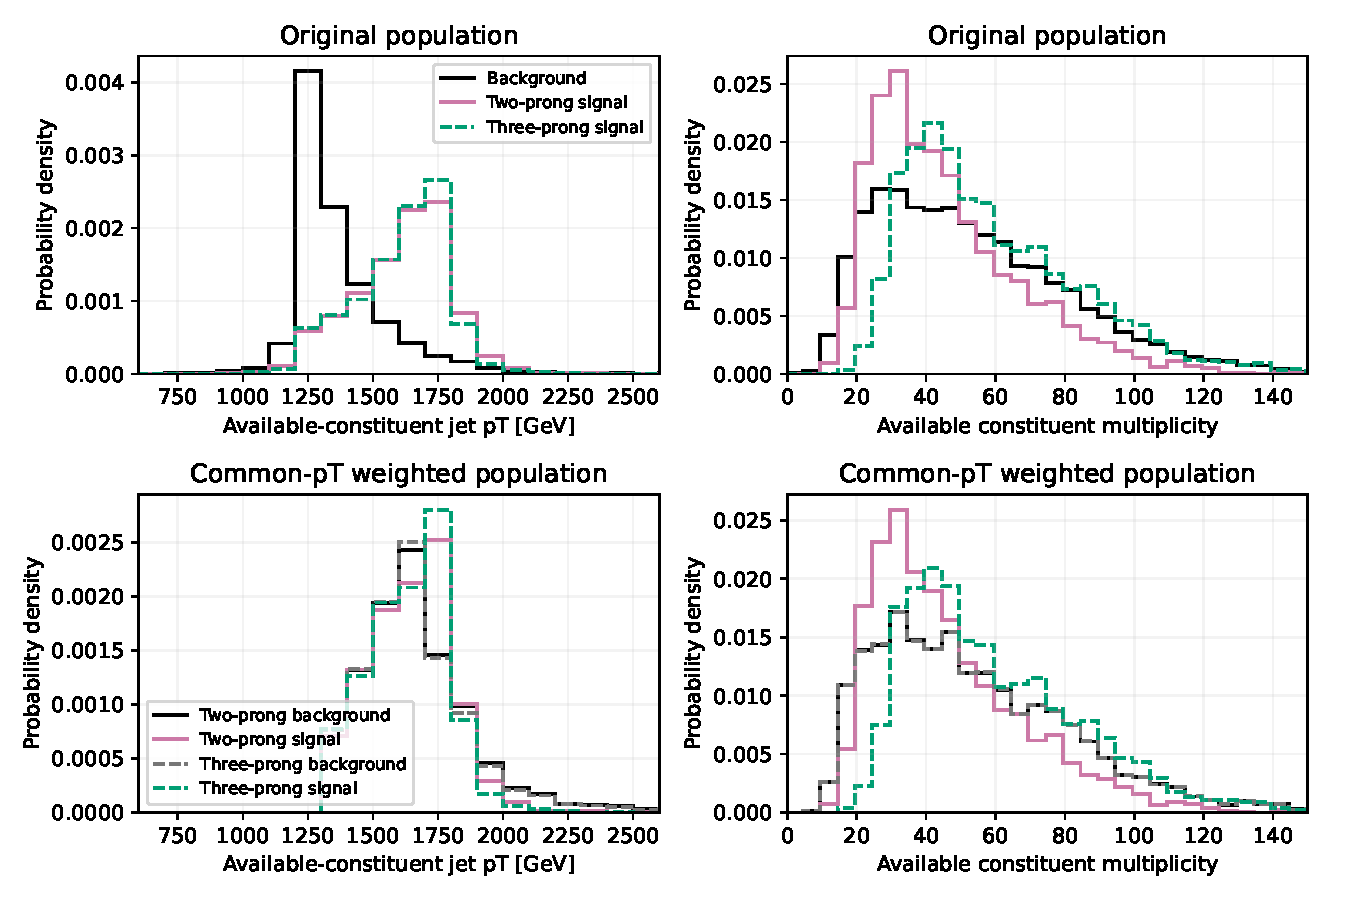
\includegraphics[width=.95\linewidth]{figures/signal_kinematics.pdf}
\caption{Momentum and available constituent multiplicity for the already-evaluated
queries, before and after the existing common-momentum weighting. Original
background events are shared across topologies; balanced background weights depend
on the signal topology. Histograms use full-population normalization, including
any probability outside the displayed range in the numerical supplement.
No new selection or model tuning is performed.}
\label{fig:signal_kinematics}\end{figure}

For background-reference covariance eigenvalues $\lambda_j$, define
$p_j=\lambda_j/\sum_k\lambda_k$ and entropy effective rank
$r_{\mathrm{eff}}=\exp[-\sum_{p_j>0}p_j\log p_j]$.
Aspen ranks are 6.11--7.65, simulation 15.25--17.10 and random 3.20--3.99
(Fig.~\ref{fig:representation}). Both trained families have higher effective
rank than their random controls. Concentrated variance alone neither establishes
pathological collapse nor explains the differential whitening gains.
Dimensional collapse can occur in contrastive learning~\cite{collapse}, but an
effective rank below 128 is not, by itself, evidence of that training pathology.
Reference/query spectra, participation ranks and correlations for all scorers
are supplied, without correlation-significance claims.

A complementary single-seed development check gives mean five-fold supervised
linear-probe balanced AUCs 0.8516 (Aspen), 0.8691 (simulation) and 0.8036 (random).
Thus information accessible to a label-trained readout can coexist with weak
background-only kNN ranking. These probes use labels and do not establish
unsupervised discovery performance; details are in the appendix. The three-prong
inversion means that signal tends to receive smaller distances to the background
reference set under this metric. It is not a statement about physical probability
density, and reversing the score after seeing labels is not an independent remedy.
\begin{figure}[htbp]\centering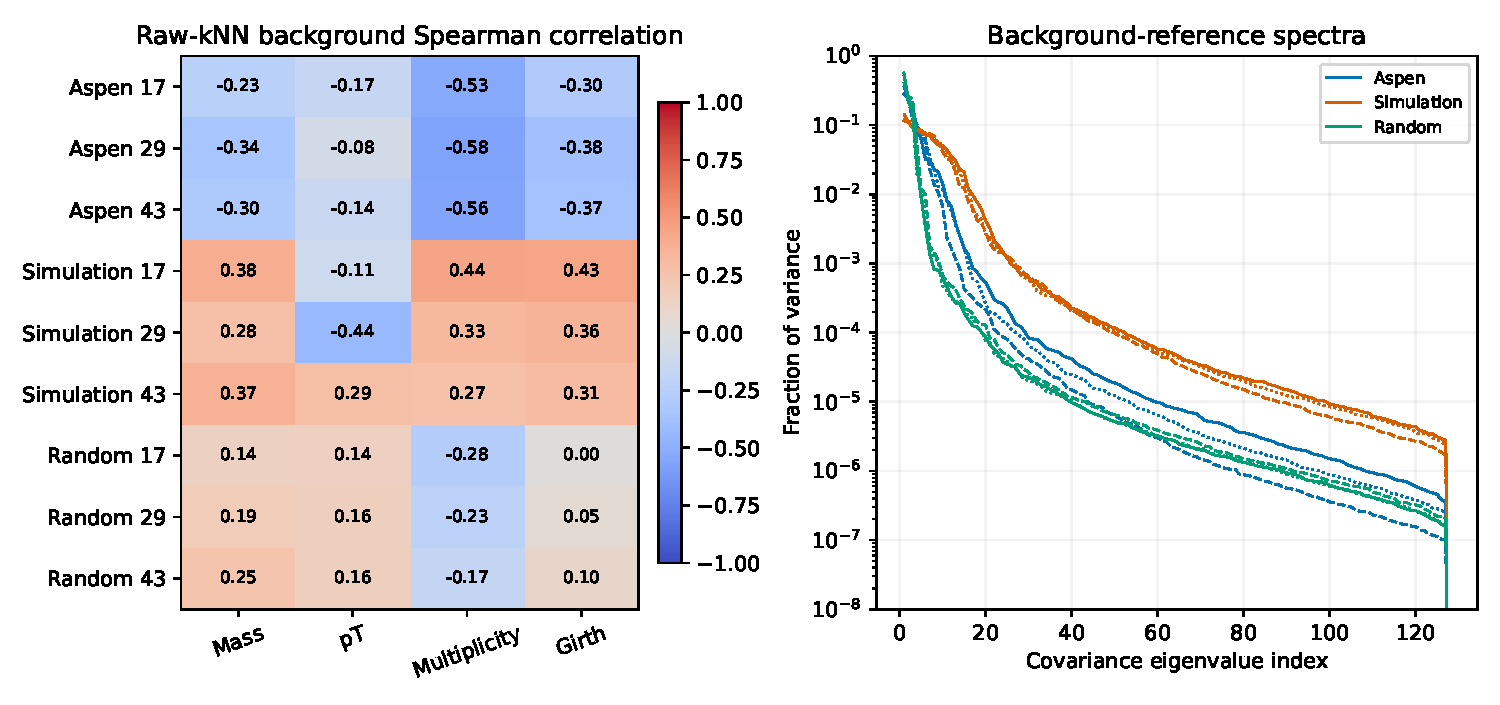
\includegraphics[width=.98\linewidth]{figures/representation_diagnostics.pdf}
\caption{Post-hoc raw-score background correlations and reference covariance
spectra for every seed. Spectral line styles indicate seeds 17 (solid), 29 (dashed)
and 43 (dotted). Eigenvalues are normalized within each model; display range is
limited to $10^{-8}$--1, while full spectra are supplied.}
\label{fig:representation}\end{figure}

\section{Limitations}
This study compares two concrete data distributions. Domain identity is confounded
with physics mixture, selection, detector response, pileup and kinematic support;
a causal effect of ``realness'' is not identified. Section~\ref{sec:support}
quantifies the large momentum mismatch but does not remove it. It uses one real-data shard,
100,000 training jets per domain, three seeds, two related simulated topologies,
one architecture and a small fixed set of scorers. It is not a result about all
real-data pretraining, foundation models or contrastive objectives.

Momentum-matched pretraining or a controlled scale-feature ablation would be needed
to test the role of the measured mismatch. Extrapolating the 24/100,000 overlap
fraction to the full Aspen collection assumes shard representativeness, which
has not been established. Counting the full available training shard yields only
350 jets from 243 events in the reference central 90\% momentum range; a
large, event-independent matched sample requires additional data. More seeds,
a full JetCLR augmentation comparison and a
mass-decorrelated girth control remain untested extensions.

Development and prior access to public benchmarks limit independence. The scorer,
operating-point and representation studies were performed after the primary
evaluation and are descriptive. Event intervals
condition on fixed models/reference fits; three seeds give limited information
about optimization variability. The paired two-prong domain-difference seed SD
of 0.104 does not permit a precise conclusion about differences of a few hundredths
with only three seeds; no equivalence or post-hoc power claim is made. No multiple-comparison discovery claim is
made. The mass-distortion analysis does not implement a background-estimation
procedure or experimental resonance search. A negative result in this setting
is informative only within these limits.

\section{Conclusion}
Equal-budget contrastive pretraining on real jets does not demonstrate a robust
anomaly-ranking advantage in this transfer configuration of 100,000 jets per
domain, one real-data shard and three seeds. The training momentum mismatch
precludes attributing this result to realness alone. Domain rankings vary
with seed, and matched random controls change the interpretation of covariance
scoring gains. Physics observables attain stronger signal retention but can
strongly reshape background jet mass; reduced distortion of the Aspen scores
comes with poor retention. The contribution is a reproducible, bounded comparison
of representation, scorer, population and operating-point behavior. These
results motivate careful evaluation of transfer representations without implying
a new anomaly-detection method or a validated search.

\section*{Data and computational artifacts}
The source datasets are public~\cite{aspen,lhco}. The accompanying reproducibility package
contains the numerical tables, machine-readable result summaries, frozen protocols,
configuration files, analysis source and provenance manifests. The full raw data
and model checkpoints are not embedded in the manuscript source archive. The
code and configuration archive is prepared for release; a public repository for
this version and model checkpoints are not yet available. Reproduction instructions
identify the required source files and computational stages; exact trained-state
reproduction can depend on the GPU/software environment. Saved scores reproduce
the numerical tables and figures; regenerating model scores requires the recorded
checkpoints or retraining with the documented procedure.

\appendix
\section{Supporting training and representation checks}\label{app:diagnostics}
Table~\ref{tab:diagnostics} reports all primary background correlations and
effective ranks. The leading-jet signal mass plot describes reconstructed
populations, not a truth assignment to $X$ or $Y$. Fixed-view validation histories
show the recorded endpoints, not an AUC-based stopping criterion. These checks
were performed after the final evaluation and are interpreted descriptively.
\begin{table}[htbp]\centering\small\begin{tabular}{lrrrrrr}
\toprule
Backbone & Seed & $\rho_m$ & $\rho_{p_T}$ & $\rho_n$ & $\rho_g$ & $r_{\mathrm{eff}}$ \\
\midrule
Aspen & 17 & -0.234 & -0.169 & -0.532 & -0.302 & 7.54 \\
Aspen & 29 & -0.340 & -0.075 & -0.578 & -0.381 & 6.11 \\
Aspen & 43 & -0.305 & -0.143 & -0.557 & -0.366 & 7.65 \\
Simulation & 17 & 0.384 & -0.114 & 0.445 & 0.431 & 17.10 \\
Simulation & 29 & 0.280 & -0.436 & 0.327 & 0.358 & 15.25 \\
Simulation & 43 & 0.370 & 0.289 & 0.270 & 0.309 & 16.01 \\
Random & 17 & 0.137 & 0.144 & -0.278 & 0.003 & 3.20 \\
Random & 29 & 0.187 & 0.158 & -0.231 & 0.054 & 3.99 \\
Random & 43 & 0.245 & 0.161 & -0.172 & 0.101 & 3.33 \\
\bottomrule
\end{tabular}

\caption{Raw-kNN background Spearman correlations and background-reference entropy
effective rank. $n$ is available multiplicity and $g$ retained-constituent girth.}
\label{tab:diagnostics}\end{table}
\begin{figure}[htbp]\centering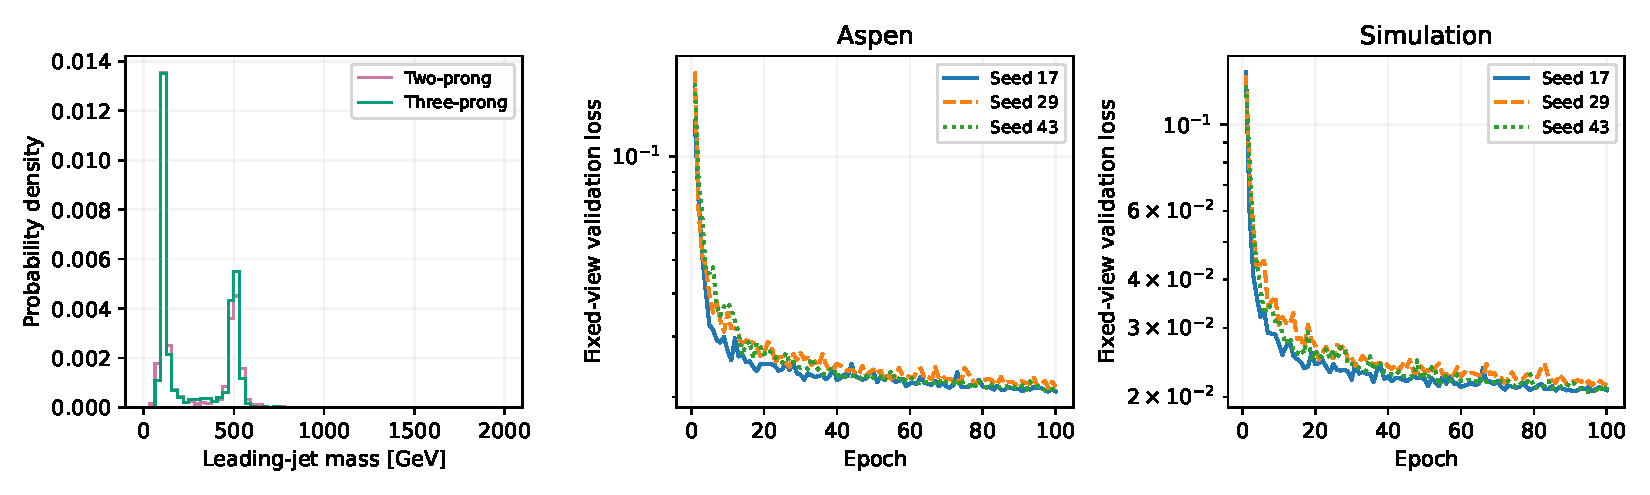
\includegraphics[width=\linewidth]{figures/signal_mass_losses.pdf}
\caption{Already-scored leading signal jet masses and recorded fixed-view validation
losses for the six trained models. No truth $X/Y$ fraction is inferred.}
\end{figure}

\section{Additional development results}
Development raw kNN mean common-$\pt$ AUCs were $0.5217\pm0.0388$ for Aspen,
$0.5562\pm0.0737$ for simulation and $0.5139\pm0.0162$ for random features.
Single-seed supervised probes gave mean five-fold balanced AUCs 0.8516, 0.8691,
0.8036 and 0.8502 for Aspen, simulation, random and four-observable inputs.
Five shared stratified folds used seed 20261002. Per-fold feature standardization
and background-reference-defined class-balancing weights were fitted on training
folds only; scikit-learn logistic regression~\cite{sklearn} used L2 regularization $C=1$, an unpenalized
intercept, LBFGS tolerance $10^{-8}$ and at most 2,000 iterations. Held-out-fold
predictions defined fold AUCs. These label-using readouts diagnose accessible
information, not background-only anomaly sensitivity. Fold spreads are not
independent training uncertainty.

A 200-epoch single-seed Aspen constituent autoencoder gave development balanced
AUCs about 0.494 for latent kNN and 0.474 for reconstruction error. It is contextual,
not a budget-matched objective comparison. Positive collinear-splitting and soft
angular-noise ablations, and a single-seed metric screen, did not justify
further compute under development triage rules. Such rules do not statistically
reject the usefulness of these methods. These exploratory arms are not selected
for the primary final comparison.

\section{Deterministic sampling and numerical checks}
Hash partitions use BLAKE2b with namespace, event identity and seed 20260925;
the 64-bit digest modulo 10,000 determines the partition. Initially inspected
events enter validation only. Source-row qqq identities are negative one minus row
index, in a separate namespace. Training sampling seed is 20260925. Final sample
indices are sorted without-replacement choices from each partition with NumPy
\texttt{default\_rng(20261004)}. Physics calibration/assessment indices use
\texttt{default\_rng(20261006).permutation(10000)}. Its threshold-refitting bootstrap
uses seed 20261007 and random-selection reference bands seed 20261008. Primary
final AUC bootstraps use seed 20261003; subsequent scorer bootstraps use 20261005.

Source and checkpoint SHA256 manifests, completed-epoch histories, finite weights,
paired initializations, fixed sample provenance and partition separation were
checked. Raw scores were reproduced from cached embeddings. Independent
float64 distances and linear-system quadratic forms checked covariance scoring;
rank-based and weighted-pair calculations checked AUC. Physics checks reproduced
thresholds, selected counts, KS and JSD with independent implementations, including
ties and bootstrap duplicates. Saved arrays retain all 1,000 bootstrap replicates.
Numerical checks establish implementation consistency, not protection against
all scientific misspecification.

\clearpage
\section{Complete seed and operating-point tables}\label{app:tables}
\begin{table}[htbp]\centering\scriptsize
\resizebox{\linewidth}{!}{\begin{tabular}{llrrrrr}
\toprule
Backbone & Scorer & Seed & 2p original & 2p balanced & 3p original & 3p balanced \\
\midrule
Aspen & Raw kNN & 17 & 0.4607 & 0.5092 & 0.3592 & 0.4005 \\
Aspen & Raw kNN & 29 & 0.5814 & 0.5844 & 0.4579 & 0.4554 \\
Aspen & Raw kNN & 43 & 0.4920 & 0.5284 & 0.3733 & 0.4005 \\
Aspen & Mahalanobis & 17 & 0.4412 & 0.5220 & 0.3475 & 0.4261 \\
Aspen & Mahalanobis & 29 & 0.5068 & 0.5255 & 0.4059 & 0.4219 \\
Aspen & Mahalanobis & 43 & 0.4513 & 0.5071 & 0.3499 & 0.4006 \\
Aspen & Whitened kNN & 17 & 0.4704 & 0.5335 & 0.3484 & 0.4040 \\
Aspen & Whitened kNN & 29 & 0.5686 & 0.5682 & 0.4448 & 0.4359 \\
Aspen & Whitened kNN & 43 & 0.4842 & 0.5260 & 0.3596 & 0.3904 \\
Simulation & Raw kNN & 17 & 0.6098 & 0.5881 & 0.6074 & 0.5874 \\
Simulation & Raw kNN & 29 & 0.3099 & 0.4879 & 0.2981 & 0.4561 \\
Simulation & Raw kNN & 43 & 0.7315 & 0.6156 & 0.7284 & 0.6147 \\
Simulation & Mahalanobis & 17 & 0.5950 & 0.5689 & 0.5889 & 0.5694 \\
Simulation & Mahalanobis & 29 & 0.3502 & 0.4841 & 0.3342 & 0.4643 \\
Simulation & Mahalanobis & 43 & 0.7213 & 0.6244 & 0.7325 & 0.6451 \\
Simulation & Whitened kNN & 17 & 0.6021 & 0.5898 & 0.5889 & 0.5812 \\
Simulation & Whitened kNN & 29 & 0.3533 & 0.5115 & 0.3331 & 0.4743 \\
Simulation & Whitened kNN & 43 & 0.7404 & 0.6535 & 0.7393 & 0.6540 \\
Random & Raw kNN & 17 & 0.6252 & 0.5090 & 0.5402 & 0.4092 \\
Random & Raw kNN & 29 & 0.6549 & 0.5372 & 0.5736 & 0.4413 \\
Random & Raw kNN & 43 & 0.6280 & 0.5054 & 0.5601 & 0.4260 \\
Random & Mahalanobis & 17 & 0.6372 & 0.5426 & 0.5551 & 0.4505 \\
Random & Mahalanobis & 29 & 0.6450 & 0.5582 & 0.5678 & 0.4751 \\
Random & Mahalanobis & 43 & 0.6277 & 0.5380 & 0.5564 & 0.4613 \\
Random & Whitened kNN & 17 & 0.6315 & 0.5635 & 0.5382 & 0.4656 \\
Random & Whitened kNN & 29 & 0.6426 & 0.5778 & 0.5526 & 0.4846 \\
Random & Whitened kNN & 43 & 0.6147 & 0.5514 & 0.5351 & 0.4697 \\
\bottomrule
\end{tabular}
}
\caption{All model/scorer seed AUCs. The corresponding CSV preserves numerical
precision. The balanced columns use the restricted common-$\pt$ population.}
\end{table}
\clearpage
\begin{table}[htbp]\centering\scriptsize
\resizebox{\linewidth}{!}{\begin{tabular}{llrrrrr}
\toprule
Backbone & Scorer & BG (\%) & 2p (\%) & 3p (\%) & KS & JSD \\
\midrule
Aspen & Raw kNN & $10.247\pm0.121$ & $7.167\pm2.816$ & $2.450\pm1.344$ & $0.129\pm0.077$ & $0.015\pm0.013$ \\
Aspen & Mahalanobis & $10.093\pm0.551$ & $6.167\pm1.533$ & $2.067\pm1.020$ & $0.135\pm0.040$ & $0.018\pm0.007$ \\
Aspen & Whitened kNN & $9.973\pm0.050$ & $6.150\pm1.621$ & $1.867\pm0.909$ & $0.127\pm0.073$ & $0.017\pm0.013$ \\
Simulation & Raw kNN & $9.920\pm0.352$ & $17.683\pm13.365$ & $18.000\pm13.141$ & $0.283\pm0.058$ & $0.055\pm0.020$ \\
Simulation & Mahalanobis & $10.053\pm0.281$ & $14.633\pm9.540$ & $15.450\pm11.616$ & $0.257\pm0.030$ & $0.048\pm0.015$ \\
Simulation & Whitened kNN & $9.707\pm0.167$ & $16.850\pm11.394$ & $16.300\pm12.229$ & $0.263\pm0.039$ & $0.050\pm0.015$ \\
Random & Raw kNN & $10.167\pm0.031$ & $16.567\pm1.492$ & $7.950\pm1.276$ & $0.251\pm0.026$ & $0.045\pm0.009$ \\
Random & Mahalanobis & $10.393\pm0.160$ & $16.450\pm1.117$ & $7.333\pm1.397$ & $0.293\pm0.037$ & $0.069\pm0.015$ \\
Random & Whitened kNN & $10.353\pm0.196$ & $22.200\pm2.693$ & $11.733\pm2.675$ & $0.327\pm0.040$ & $0.076\pm0.016$ \\
Girth & -- & 10.260 & 35.750 & 38.550 & 0.804 & 0.428 \\
Observable density & -- & 10.300 & 42.300 & 40.800 & 0.564 & 0.216 \\
\bottomrule
\end{tabular}
}
\caption{All methods at nominal 10\% background acceptance. Efficiencies are
percentages; model rows show mean $\pm$ seed SD. KS and JSD concern background
jet mass; JSD uses natural logs. Actual acceptance is measured on a disjoint
background assessment sample.}
\end{table}
\begin{table}[htbp]\centering\scriptsize
\resizebox{\linewidth}{!}{\begin{tabular}{llrrrrr}
\toprule
Backbone & Scorer & BG (\%) & 2p (\%) & 3p (\%) & KS & JSD \\
\midrule
Aspen & Raw kNN & $5.533\pm0.150$ & $3.167\pm1.329$ & $0.917\pm0.473$ & $0.135\pm0.082$ & $0.018\pm0.017$ \\
Aspen & Mahalanobis & $5.560\pm0.223$ & $3.100\pm0.577$ & $0.733\pm0.388$ & $0.158\pm0.063$ & $0.023\pm0.013$ \\
Aspen & Whitened kNN & $5.507\pm0.064$ & $2.867\pm0.679$ & $0.600\pm0.304$ & $0.145\pm0.063$ & $0.019\pm0.013$ \\
Simulation & Raw kNN & $4.947\pm0.201$ & $9.750\pm9.148$ & $9.683\pm8.590$ & $0.318\pm0.062$ & $0.068\pm0.022$ \\
Simulation & Mahalanobis & $4.880\pm0.347$ & $6.417\pm4.060$ & $7.017\pm5.312$ & $0.279\pm0.043$ & $0.058\pm0.020$ \\
Simulation & Whitened kNN & $4.993\pm0.081$ & $8.567\pm6.698$ & $8.133\pm6.860$ & $0.283\pm0.053$ & $0.058\pm0.025$ \\
Random & Raw kNN & $5.267\pm0.081$ & $8.083\pm0.451$ & $3.283\pm0.076$ & $0.271\pm0.016$ & $0.055\pm0.009$ \\
Random & Mahalanobis & $5.507\pm0.076$ & $8.233\pm0.551$ & $2.950\pm0.229$ & $0.348\pm0.067$ & $0.090\pm0.027$ \\
Random & Whitened kNN & $5.693\pm0.150$ & $11.633\pm1.286$ & $4.367\pm0.679$ & $0.370\pm0.038$ & $0.090\pm0.016$ \\
Girth & -- & 4.820 & 24.100 & 22.050 & 0.893 & 0.504 \\
Observable density & -- & 4.740 & 31.850 & 30.300 & 0.586 & 0.244 \\
\bottomrule
\end{tabular}
}
\caption{As above at nominal 5\%. Full per-seed thresholds, counts, Wilson intervals,
threshold-refitting bootstrap intervals, mass/$\pt$ profiles and paired differences
are supplied in the machine-readable numerical supplement.}
\end{table}
\clearpage
\begin{thebibliography}{99}
\bibitem{jetclr} B. M. Dillon, G. Kasieczka, H. Olischlager, T. Plehn, P. Sorrenson and L. Vogel,
Symmetries, Safety, and Self-Supervision, SciPost Phys. 12, 188 (2022),
\href{https://arxiv.org/abs/2108.04253}{arXiv:2108.04253}.
\bibitem{dillon2022} B. M. Dillon, R. Mastandrea and B. Nachman,
Self-supervised Anomaly Detection for New Physics, Phys. Rev. D 106, 056005 (2022),
\href{https://arxiv.org/abs/2205.10380}{arXiv:2205.10380}.
\bibitem{anomalyclr} B. M. Dillon, L. Favaro, F. Feiden, T. Modak and T. Plehn,
Anomalies, Representations, and Self-Supervision, SciPost Phys. Core 7, 056 (2024),
\href{https://arxiv.org/abs/2301.04660}{arXiv:2301.04660}.
\bibitem{aspen} O. Amram et al., Aspen Open Jets: Unlocking LHC Data for Foundation
Models in Particle Physics, Mach. Learn. Sci. Technol. 6, 030601 (2025),
\href{https://arxiv.org/abs/2412.10504}{arXiv:2412.10504}.
\bibitem{omnilearned} W. Bhimji, C. Harris, V. Mikuni and B. Nachman,
OmniLearned: A Foundation Model Framework for All Tasks Involving Jet Physics,
Phys. Rev. D 113, 032020 (2026),
\href{https://arxiv.org/abs/2510.24066}{arXiv:2510.24066}.
\bibitem{metzger} K. Metzger et al., Anomaly preserving contrastive neural embeddings
for end-to-end model-independent searches at the LHC,
Phys. Rev. D 112, 072011 (2025),
\href{https://arxiv.org/abs/2502.15926}{arXiv:2502.15926}.
\bibitem{omnijet} J. Birk, A. Hallin and G. Kasieczka,
OmniJet-$\alpha$: The first cross-task foundation model for particle physics,
Mach. Learn. Sci. Technol. 5, 035031 (2024),
\href{https://arxiv.org/abs/2403.05618}{arXiv:2403.05618}.
\bibitem{ddt} J. Dolen, P. Harris, S. Marzani, S. Rappoccio and N. Tran,
Thinking outside the ROCs: Designing Decorrelated Taggers (DDT) for jet
substructure, JHEP 05 (2016) 156,
\href{https://arxiv.org/abs/1603.00027}{arXiv:1603.00027}.
\bibitem{massive} T. Golling et al., The Mass-ive Issue: Anomaly Detection in Jet Physics,
\href{https://arxiv.org/abs/2303.14134}{arXiv:2303.14134} (2023).
\bibitem{lhco} G. Kasieczka, B. Nachman and D. Shih,
R\&D Dataset for LHC Olympics 2020 Anomaly Detection Challenge, version 5,
Zenodo (2022), \href{https://doi.org/10.5281/zenodo.6466204}{doi:10.5281/zenodo.6466204}.
\bibitem{lhcocommunity} G. Kasieczka et al., The LHC Olympics 2020: A Community
Challenge for Anomaly Detection in High Energy Physics,
Rep. Prog. Phys. 84, 124201 (2021),
\href{https://doi.org/10.1088/1361-6633/ac36b9}{doi:10.1088/1361-6633/ac36b9},
\href{https://arxiv.org/abs/2101.08320}{arXiv:2101.08320}.
\bibitem{antikt} M. Cacciari, G. P. Salam and G. Soyez,
The anti-$k_t$ jet clustering algorithm, JHEP 04 (2008) 063,
\href{https://arxiv.org/abs/0802.1189}{arXiv:0802.1189}.
\bibitem{fastjet} M. Cacciari, G. P. Salam and G. Soyez,
FastJet user manual, Eur. Phys. J. C 72, 1896 (2012),
\href{https://arxiv.org/abs/1111.6097}{arXiv:1111.6097}.
\bibitem{attention} A. Vaswani et al., Attention Is All You Need,
Adv. Neural Inf. Process. Syst. 30 (2017),
\href{https://arxiv.org/abs/1706.03762}{arXiv:1706.03762}.
\bibitem{simclr} T. Chen, S. Kornblith, M. Norouzi and G. Hinton,
A Simple Framework for Contrastive Learning of Visual Representations,
Proc. 37th Int. Conf. Mach. Learn., PMLR 119, 1597--1607 (2020),
\href{https://arxiv.org/abs/2002.05709}{arXiv:2002.05709}.
\bibitem{adamw} I. Loshchilov and F. Hutter, Decoupled Weight Decay Regularization,
ICLR (2019), \href{https://arxiv.org/abs/1711.05101}{arXiv:1711.05101}.
\bibitem{wilson} E. B. Wilson, Probable Inference, the Law of Succession, and Statistical
Inference, J. Amer. Statist. Assoc. 22, 209--212 (1927),
\href{https://doi.org/10.1080/01621459.1927.10502953}{doi:10.1080/01621459.1927.10502953}.
\bibitem{sklearn} F. Pedregosa et al., Scikit-learn: Machine Learning in Python,
J. Mach. Learn. Res. 12, 2825--2830 (2011),
\url{https://www.jmlr.org/papers/v12/pedregosa11a.html}.
\bibitem{rs3l} P. Harris, M. Kagan, J. Krupa, B. Maier and N. Woodward,
Re-Simulation-based Self-Supervised Learning for Pre-Training Foundation Models,
Phys. Rev. D 111, 032010 (2025),
\href{https://arxiv.org/abs/2403.07066}{arXiv:2403.07066}.
\bibitem{mpm} T. Golling et al., Masked Particle Modeling on Sets: Towards
Self-Supervised High Energy Physics Foundation Models,
Mach. Learn. Sci. Technol. 5, 035074 (2024),
\href{https://arxiv.org/abs/2401.13537}{arXiv:2401.13537}.
\bibitem{disco} G. Kasieczka and D. Shih,
DisCo Fever: Robust Networks Through Distance Correlation,
Phys. Rev. Lett. 125, 122001 (2020),
\href{https://arxiv.org/abs/2001.05310}{arXiv:2001.05310}.
\bibitem{collapse} L. Jing, P. Vincent, Y. LeCun and Y. Tian,
Understanding Dimensional Collapse in Contrastive Self-supervised Learning,
ICLR (2022), \href{https://arxiv.org/abs/2110.09348}{arXiv:2110.09348}.
\end{thebibliography}

\end{document}
